\documentclass{standalone}

\usepackage{tikz}

\begin{document}
	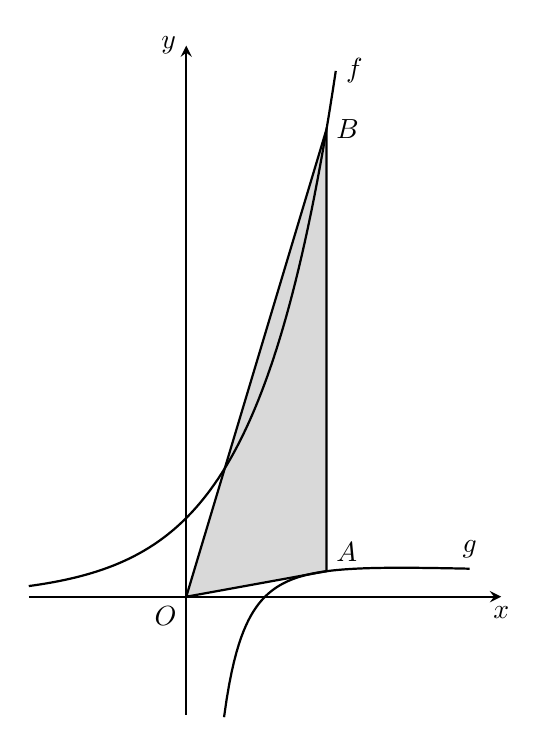
\begin{tikzpicture}
		\coordinate (O) at (0,0);
		\coordinate (A) at (1.781, 0.324);
		\coordinate (B) at (1.781, 5.936);		
		\draw[thick, fill=gray!30] (O) -- (A) -- (B) -- cycle;
		\draw [thick, domain=-2:1.9, samples=100] plot (\x, {e^\x}) node[right]{\(f\)};
		\draw [thick, domain=0.48:3.6, samples=100] plot (\x, {ln(\x)/(\x)}) node[above]{\(g\)};
		\draw[thick, -> , >=stealth](-2,0) -- (4,0) node[below]{\(x\)};
		\draw[thick, -> , >=stealth](0,-1.5) -- (0,7) node[left]{\(y\)};
		\draw (O) node[below left]{\(O\)};
		\draw (A) node[above right]{\(A\)};
		\draw (B) node[right]{\(B\)};
	\end{tikzpicture}
\end{document}